\documentclass[runningheads]{llncs}

%---- Sonderzeichen-------%
\usepackage[ngerman]{babel}
%---- Codierung----%
\usepackage[utf8]{inputenc}
%\usepackage[latin1]{inputenc}
\usepackage[T1]{fontenc}
\usepackage{graphicx}
\usepackage{url}
\usepackage{llncsdoc}
%----- Mathematischer Zeichenvorrat---%
\usepackage{amsmath}
\usepackage{amssymb}
\usepackage{enumerate}
% fuer die aktuelle Zeit
\usepackage{scrtime}
\usepackage{listings}
\usepackage{subfigure}
\usepackage{hyperref}

\setcounter{tocdepth}{3}
\setcounter{secnumdepth}{3}

% -------------------------------------------------------------------------------------------------
% -------------------------------------------------------------------------------------------------

\mainmatter
\title{Universal Rendering}
\titlerunning{Universal Rendering}
\author{Julian Beck}
\authorrunning{Julian Beck}
\institute{Betreuer: Prof. Dr. rer. nat. Christian Zirpins}
\date{01.05.2019}
\begin{document}
\let\oldaddcontentsline\addcontentsline
\def\addcontentsline#1#2#3{}
\maketitle
\def\addcontentsline#1#2#3{\oldaddcontentsline{#1}{#2}{#3}}

% -------------------------------------------------------------------------------------------------

\begin{abstract}
  An dieser Stelle sollte später eine Kurzzusammenfassung stehen.
\end{abstract}

% -------------------------------------------------------------------------------------------------
\tableofcontents 
\newpage
% -------------------------------------------------------------------------------------------------

\section{Einleitung}
\label{sec:Einleitung}

Seit dem Beginn des Webs funktioniert das Surfen wie folgt: 
Ein Webbrowser fordert eine bestimmte Seite an, ein Server im 
Internet bearbeitet die Anfrage und generiert ein HTML 
(Hypertext Markup Language) Dokument als Antwort. 
Dies bezeichnet man als serverseitiges rendern. 
In den Anfängen des Webs stellte dies kein Problem dar, 
da die Browser nicht leistungsstark waren und die Webseiten 
aus meist statischen Inhalt bestanden. 
Später mit HTML5 wurden Webseiten dynamischer und 
interaktiver für den Nutzer, was dazu führte, dass immer mehr Apps, 
sogenannte Single Page Applikationen, 
vollständig im Browser auf einer Seite liefen. 
Um dies zu ermöglichen wird clientseitiges rendern verwendet. 
Single Page Applications oder kurz SPAs, bieten Vorteile für den Anwender: 
Sie reagieren schnell auf Benutzerinteraktionen und können zwischen Seiten navigieren, 
ohne sie komplett neu zu laden. Gleichzeitig sind SPAs komfortabel zu entwickeln, 
dank moderner Frameworks. Beide Varianten, serverseitiges und clientseitiges rendern, 
haben Vor- und Nachteile. Universal Rendering kombiniert die beiden Ansätze und 
erfüllt alle Anforderungen an eine moderne Webanwendung.


\subsection{Anforderungen an eine Webanwendung}
\label{subsec:Anforderungen an eine Webanwendung}

Eine moderne Webanwendungen sollten folgende Anforderungen erfüllen:
\begin{itemize}
  \item Damit die Seite von Suchmaschinen gefunden werden kann, sollte sie von Suchmaschinen Crawler indexierbar sein. 
  Dies wird Suchmaschinenoptimierung oder auch SEO 
  (engl. search engine optimization) genannt. 
  \item Eine moderne Webseite muss beim Aufrufen für den Anwender schnell laden. Der Anwender sollte nicht lange warten 
  müssen bis er die Anwendung sieht und mit ihr interagieren kann
  \item Eine moderne Webanwendung muss dynamisch und interaktiv sein. Die Anwendung sollte auf Benutzereingaben reagieren, 
  ohne lange Ladezeiten oder neuladen der Seite.
  Die Anwendung sollte einfach zu entwickeln sein und gleichzeitig muss sichergestellt werden, 
  dass der Programmcode einfach zu pflegen ist. 
  Code duplikation sollte minimiert werden.
\end{itemize}

\subsection{Terminologie}
\label{subsec:Terminologie}
Beim Rendern von Webtechnologien unterscheidet man zwischen dem Rendern auf dem Server und dem Client:

\begin{itemize}
  \item SSR Server-Side Rendering: Rendern auf der Server Seite bezieht sich auf das generieren eines HTML Dokumentes 
  aus einer Single Page Application. 
  \item CSR Client-Side Rendering: Rendern auf der Client Seite bezieht sich auf das generieren und parsen eines 
  HTML Dokumentes zu einem DOM und darstellen für den Anwender. 
\end{itemize}
Der Begriff Universal Rendering beschreibt eine Kombination aus server- und clientseitiges rendern. 
Dieser Ansatz wird oft auch als Isomorphic oder Server-Side Rendering bezeichnet.

Folgende Begriffe beschreiben unterschiedliche Zeiten beim Laden einer Webseite:
\begin{itemize}
  \item TTFB: Time to First Byte - Zeit bis zum ersten Byte -  Die Zeit zwischen dem Klicken auf ein Link und Erhalten der Daten vom Server.
  \item FP: First Paint - der Zeitpunkt an dem der erste Inhalt für den User sichtbar wird.
  \item FCP: First Contentful Paint oder auch First Meaningful Paint - Der Zeitpunkt, an dem der Benutzer den wichtigsten Inhalt einer Website als fertig geladen sieht. Die Zeit bis zum FCP wird auch als kritischer Rendering-Pfad (engl.:Critical Rendering Path) bezeichnet.
  \item TTI: Time To Interactive - Die Zeit bis die Seite interaktiv wird und der Anwender mit ihr interagieren kann.
\end{itemize}
Da die Anwendung vollständig auf der Client Seite läuft, ist es schwierig für Suchmaschinen Crawler die seite zu Indexieren was zu einer schlechten SEO führt.
Des weiteren, dadurch dass die Webseite nicht auf dem Server, sonder vom Client gerendert wird, muss der User warten bis die seite vollständig gerendert wird.
Server Side rendering ist eine Mischung beider Ansätze. Es kombiniert die SEO und Performance von Server seitigen Applikationen und die Interaktivität und flexibilität von Client Side Anwendungen.

Diese Arbeit beginnt mit den der Funktionsweise von server - und clientseitigen Rendern. 
Es werden die Vor - und Nachteile der jeweiligen Vorgehensweisen untersucht 
und beschrieben warum eine Notwendigkeit für Universal Rendering besteht. Nach einer Einführung in den Universal Rendering Vorgang, werden die verwendeten Technologien und deren Funktionsweise für das Rendern beschrieben. Anschließend werden die positiven und negativen Aspekte des Universal Rendering beschrieben und Alternativen genannt. Danach beschreibt die Arbeit unterschiedliche Frameworks zum implementieren der Rendering Technologie und zeigt wie Unternehmen Universal Rendering verwenden. Das Fazit erarbeitet wann welche Rendering Technologie verwendet werden soll und zeigt den aktuellen Stand von Suchmaschinen Crawler.
\newpage
% -------------------------------------------------------------------------------------------------

\section{Serverseitiges Rendering}
\label{sec:Serverseitiges Rendering}
Bei der klassische Web-Architektur oder auch “Thin Client - Fat Server” 
Architektur, befindet sich die Anwendungslogik auf der Serverseite. 
Diese Logik wird durch Programmiersprachen wie PHP, Python oder Java 
implementiert. Die Clientseite ist nur zuständig für die “Document Object Model” 
Manipulation und dem Darstellen der Webseite im Browser.
\begin{figure}[h]
  \centering
  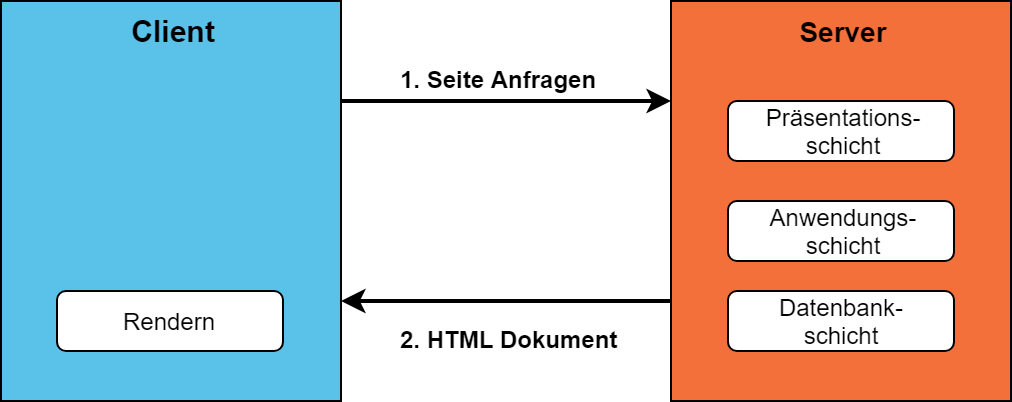
\includegraphics[width=12cm]{images/server}
  \caption{Thin Client - Fat Server Architektur einer SSR Anwendung}
  \label{Thin Client - Fat Server Architektur einer SSR Anwendung}
\end{figure}

Wird eine Website aufgerufen, wird zunächst über das HTTP Protokoll 
eine GET Anfrage an den Server gesendet. Dieser bearbeitet die Anfrage 
und antwortet mit einem HTML Dokument. Auf der Clientseite wird das HTML 
von dem Browser interpretiert und dargestellt.

Der kritische Rendering-Pfad ist bei klassischen Webanwendungen sehr schnell, 
da das HTML vom Server gerendert wird. Dies bietet eine gute Nutzererfahrung, 
da der Client ausschließlich die Webseite als DOM darzustellen muss. 
Beim Erhalten der Antwort, sieht der Anwender schon den First Contentful Paint 
und kann mit der Seite interagieren. Damit ist die Zeit bis zum FCP gleich lang, 
wie die Time to Interactive der Website. Dies bringt eine gute Nutzererfahrung, 
da der User sofort nach dem Laden mit der Website interagieren kann, 
anders als bei Clientseitigen Anwendungen. 
Da die Webseite direkt mit HTML antwortet, ist es einfach für Suchmaschinen Crawler 
die Webseite zu indexieren. 

Der entscheidende Nachteil von klassischen serverseitigen Anwendungen 
ist die Benutzer Interaktivität. Für jede Navigation zwischen verschiedenen 
Seiten und für jedes abgeschickte HTML-Form, 
muss eine neue Anfrage an den Server gesendet werden. 
Dies erfordert ein komplettes Neuladen der Webseite, 
auch wenn nur ein einziges Element aktualisiert werden soll. 
Da der Browser bei auf diese Art nur eine Anfrage bearbeiten kann, 
bezeichnet man dies als synchrone Kommunikation. 
Mit dem Einführen von Ajax wurden Webanwendungen asynchron, 
was zu einer besseren Nutzererfahrung führte.

\subsection{Serverseitiges Rendering mit Ajax}
\label{subsec:Serverseitiges Rendering mit Ajax}
Mit der Einführung von XMLHttpRequest von Microsoft im Jahre 2000 wurde die Basis von Ajax geschaffen. 
Ajax oder auch “asynchronous JavaScript and XML” erlaubt eine asynchrone Datenübertragung mit dem Server.
\begin{figure}[h]
  \centering
  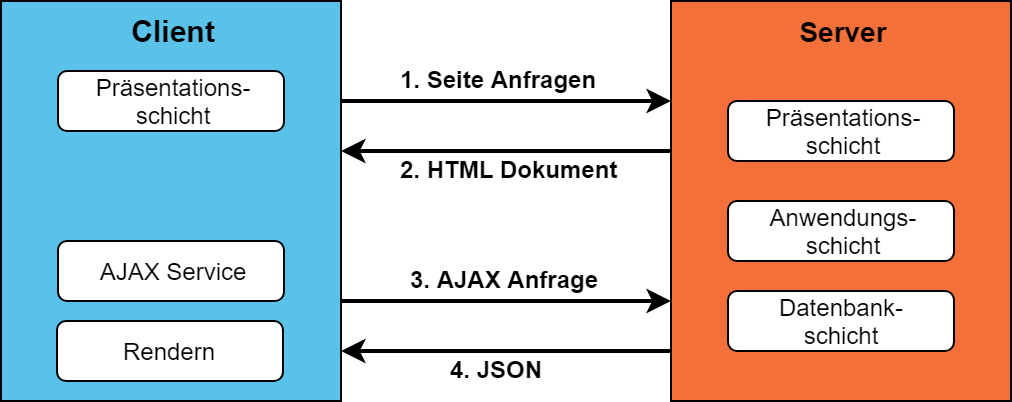
\includegraphics[width=12cm]{images/serverajax}
  \caption{HTMl Dokument einer React Seite}
\end{figure}
Ajax löst das Problem der synchronen Kommunikation klassischer Webanwendungen. 
Ajax ermöglicht es asynchron, 
den Inhalt einer Webseite zu aktualisieren und Daten zum Server senden und empfangen, 
ohne neuladen der Webseite. Damit dies möglich ist, 
kommuniziert die Clientseite, mittels Ajax, mit dem Server. 
So ist es möglich, interaktive und dynamische Webanwendungen zu bauen, 
die sofort reagieren ohne ein Neuladen der Seite.

Die Verwendung von Ajax führt aber auch zu einer komplizierten Web-Architektur. 
Zuvor war die Anwendungslogik auf der Serverseite. 
Dies erlaubte eine klare Trennung zwischen Client und Server. 
Das Aktualisieren von Teilbereichen der Webseite führt 
zu einer Verbesserung der Nutzererfahrung. 
Es erfordert aber auch doppelte Templates und erhöht den Programmanteil sowie Logik auf der Clientseite. 
Um Ajax zu benutzen ist mehr JavaScript auf der Clientseite erforderlich. 
Besitzt eine Anwendung Logik auf der Client- und Serverseite, 
wird es schwerer diese zu entwickeln. 
ie Wartbarkeit wird erhöht und es sind mehr Unittests nötig, 
die sicherstellen, dass der Zustand der Anwendung auf Server und 
Client gleich ist. 
\newpage
% -------------------------------------------------------------------------------------------------

\section{Clientseitiges Rendering}
\label{sec:Clientseitiges Rendering}

Single Page Application kurz SPAs werden durch moderne Frameworks wie React, 
Vue und Angular immer beliebter. SPAs sind komfortabel zu Entwickeln 
und lösen das Problem der Wartbarkeit, 
indem sie vollständig auf der Clientseite, 
im Browser, ausgeführt werden.

Single Page Application verwenden die ”Fat- Client, Thin Server Architektur”. 
Dabei befindet sich die Anwendungs- und Interface Logik vollständig auf der Clientseite. 
Die Serverseite ist nur zuständig für das Bereitstellen von Anwendungsdaten 
und benötigten Scripts. 
Beim Aufrufen einer Single Page Application antwortet der Server 
mit einem leeren HTML Dokument, das nur ein Template und Links 
zu den benötigten Scripts enthält. 
Der Client lädt anschließend die JavaScript Dateien runter, 
initialisiert die Anwendung und rendert das HTML im Browser. 
Damit findet das Rendern der Anwendung nur auf der Clientseite statt. 
Ist der Client initialisiert, ruft er mittels Ajax weitere Anwendungsdaten ab.

\begin{figure}[h]
  \centering
  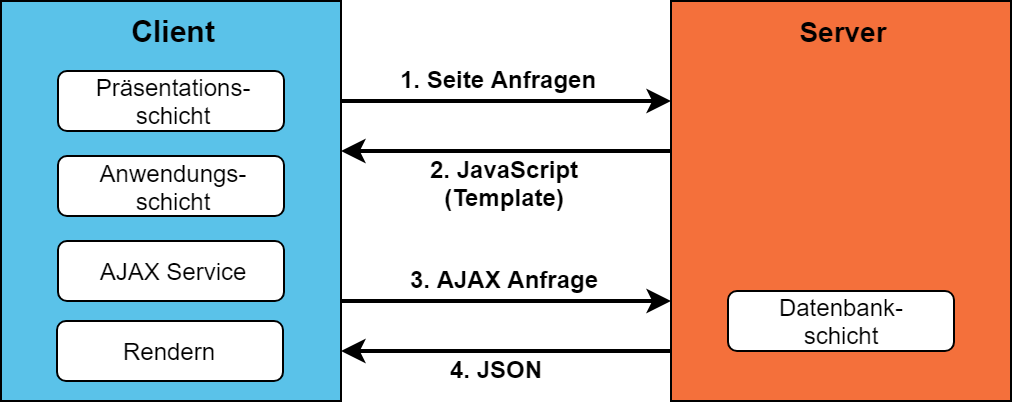
\includegraphics[width=12cm]{images/client}
  \caption{HTMl Dokument einer React Seite}
\end{figure}

Dieses Vorgehen hat Vorteile beim Wechseln zwischen einzelnen Seiten. 
Der Client muss beim Navigieren keine neue Daten vom Server anfordern, 
sondern nur den angezeigten Inhalt wechseln. 
Somit ist kein Neuladen der Seite nötig. 
Aus diesem Grund werden Single Page Apps oft bei interaktiven Anwendung, 
wie beispielsweise Googles GMAIL verwendet. 
Da die Anwendungslogik vollständig auf der Clientseite liegt, 
ist eine klare Trennung zwischen Server und Client möglich. 
Dies vereinfacht das Entwickeln von SPAs und
macht in Kombination mit modernen Frameworks 
Single Page Applications bei Entwicklern sehr beliebt.

Beim Aufrufen von serverseitig gerenderten Webseiten antwortet
der Server direkt mit einem HTML Dokument, 
dass den angeforderten Inhalt enthält. 
Bei SPAs hingegen antwortet der Server nur mit einem Template. 
Der Client lädt anschließend die JavaScript Bibliotheken, 
wie beispielsweise React und initialisiert die Webseite. 
Während dem Initialisieren kann der Anwender nicht mit der Seite interagieren
und muss warten. Oft werden Ladebalken verwendet, 
die der Benutzer sieht, bis die Seite geladen ist. 
Aus diesem Grund ist die Time to Interactive und 
der kritische Rendering-Pfad sehr hoch, im Gegensatz zu SSR.

Ein weiteres Problem mit SPAs ist die Search Engine Optimization (SEO). 
Da beim Aufrufen einer CSR Anwendung der Server nur mit einem Template 
antwortet, dass nur JavaScript und kein Inhalt enthält, 
kann es nicht von Suchmaschinen indexiert werden. 
Beim Indexieren einer React Anwendung beispielsweise, 
enthält der Crawler die in Abbildung XX enthaltene Antwort des Servers. 

\begin{figure}[h]
  \centering
  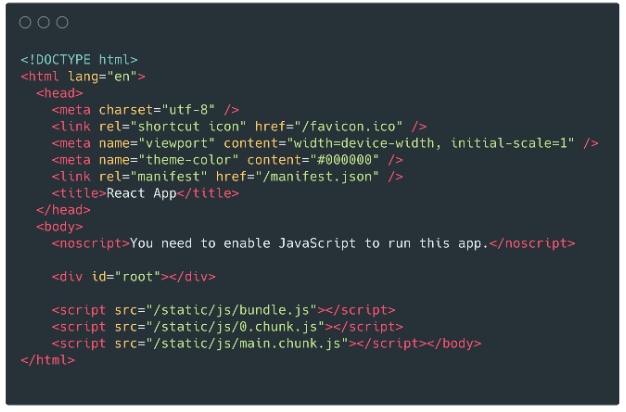
\includegraphics[width=9cm]{images/react-code-small}
  \caption{HTMl Dokument einer React Seite}
\end{figure}

Stattdessen ist notwendig, dass die Suchmaschine die Anwendung rendert, 
was nicht jeder Suchmaschinen Provider macht. 
Eine weitere Herausforderung bei der SEO sind die URLs der Anwendung. 
SPAs verwenden Hash Marks zur Navigation zwischen Seiten. 
Eine Hash Mark wird am Ende einer SPA Domain verwendet. 
Zum Beispiel würde aus einer der URL \url{https://example/test} bei einer SPA 
\url{https://example#/test} werden. 
Das Verwenden des Hash am Ende der URL verhindert, 
dass der Browser eine neue Anfrage sendet. 
Dies ist wichtig, da die Grundidee einer SPA darin besteht, 
dass nur die Daten angefordert werden, 
die zum Rendern einer Ansicht / Seite erforderlich sind, 
anstatt ein neues Dokument für jede Seite abzurufen und zu rendern. 
Für ein Web Crawler unterscheiden sich Domains mit Hash Mark allerdings 
nicht, was die Indizierung von Seiten erschwert.

Ein weiteres Problem stellt die Social Media Optimization (SMO) für SPAs dar. 
Da die Anwendung clientseitig läuft, 
können Social Media Crawler die Webseite nicht einfach crawlen, 
wie bei serverseitigen Anwendungen. Dies kann dazu führen, 
dass bei dem Verwenden von Links auf sozialen Plattformen 
keine Vorschau des Inhaltes generiert werden kann. 
Da die Inhalte nicht sehr einfach teilbar sind, 
kann dies die  Nutzerzahlen einer Anwendung beeinflussen.

Single Page Applications sind sehr dynamisch und interaktiv. 
Sie lassen sich mit Hilfe von Frameworks wie React komfortabel entwickeln
und benötigen keinen dynamischen Server. Es reicht aus, 
die Template Datei statisch bereitzustellen. 
Allerdings brauchen SPAs lange zum Laden der ersten Seite
und sind für Suchmaschinen schwer zu optimieren. 
\newpage
% -------------------------------------------------------------------------------------------------

\section{Universal Rendering}
\label{sec:Universal Rendering}
Universal rendering kombiniert serverseitiges- und clientseitiges rendern. 
Es ermöglicht SEO freundliche, interaktive Webseiten zu bauen, 
die gleichzeitig schnell auf dem Endgerät des Anwenders laden. 
Um dies zu erreichen, 
verwendet Universal Rendering die positiven Aspekte beider Technologien.

\begin{equation*}
  SSR + CSR = Universal App
\end{equation*}
\\
Beim Aufrufen einer Universal rendering Anwendung sendet der Browser
zuerst eine Anfrage an den Server. 
Dieser rendert die Anfrage und antwortet mit einem HTML Dokument. 
Ab diesem Zeitpunkt kann die Seite für den Anwender dargestellt werden, 
er erhält den First Contentful Paint (FCP). 
Anschließend lädt der Browser im Hintergrund eine Single Page Application herunter
und startet sie. 
Jetzt funktioniert die Anwendung wie eine Single Page Anwendung und 
verwendet Client Side Rendering. 
\begin{figure}[h]
  \centering
  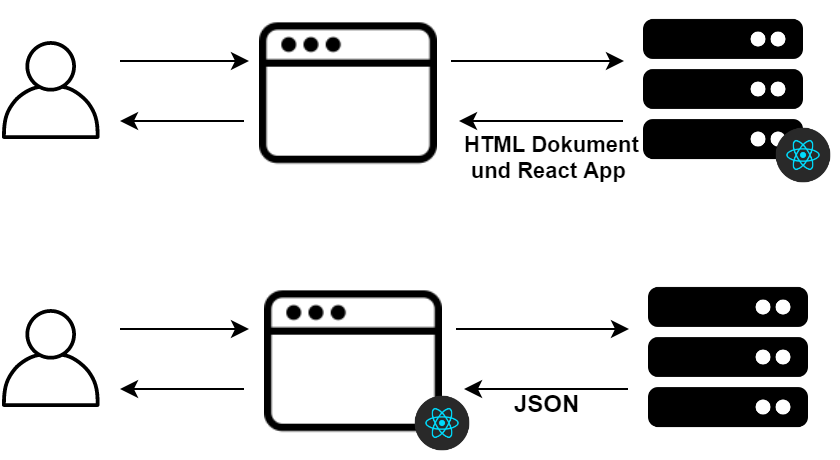
\includegraphics[width=12cm]{images/react}
  \caption{HTMl Dokument einer React Seite}
\end{figure}

Um dies zu ermöglichen kombiniert Universal Rendering mehrere Technologien. 
Es wird Isomorphic JavaScript verwendet um JavaScript auf dem Server und Client auszuführen, 
ein virtueller DOM für das Rendern auf dem Server und 
Code Hydration für den Wechsel zwischen server zu clientseitigen Rendern.

\begin{figure}[h]
  \centering
  
\includegraphics[width=10cm]{images/universalseo}
  \caption{HTMl Dokument einer React Seite}
\end{figure}

\subsection{Isomorphic JavaScript}
\label{subsec:Isomorphic JavaScript}
Isomorphic Javascript oder auch Universal Javascript genannt, 
beschreibt JavaScript Code der auf der Server- und Clientseite ausführbar ist. 
Die JavaScript Laufzeitumgebung Node.js ermöglichen dabei 
das Ausführen von JavaScript-Code auf dem Server. 
Damit erlaubt Isomorphic JavaScript, 
in Kombination mit einem virtuellen DOM, moderne clientseitige Frameworks auf der Serverseite auszuführen. 
Dies verhindert auch das Problem der Code Duplikation, 
da es möglich ist den gleichen JavaScript Code auf dem Server und Client auszuführen, 
was die Wartbarkeit und Testbarkeit verbessert.

\subsection{Virtuelles DOM}
\label{subsec:Virtuelles DOM}
Das Virtuelle Document Object Model
oder auch virtuelles DOM (eng. virtual DOM) ermöglicht 
as Rendern moderner Web Anwendungen auf dem Server.

Bei modernen JavaScript Frameworks wie React, 
VueJs und Angular wird das HTML vollständig vom Framework kontrolliert. 
So kann das Framework einfach das HTML manipulieren und stellt sicher, 
dass der Zustand (engl. state) der Anwendung gleich mit dem Interface ist. 
So kann zum Beispiel bei einer Todo List Anwendung mit React sichergestellt werden, 
dass beim Löschen einer Aufgabe der Zustand synchron mit dem Interface ist. 
Moderne JavaScript Frameworks garantieren, 
dass das Interface immer mit dem Zustand synchron ist und aktualisiert das Interface, 
sobald sich der Zustand ändert. 
Dabei wird ein virtuelles Document Object Model (virtual DOM) verwendet.

Das Document Object Model ist eine Datenstruktur in Form eines Baumes, 
die erzeugt wird, wenn der Browser das HTML Dokument rendert. 
Ein aktualisieren des Inhaltes einer Website ist nur möglich, 
durch Manipulation des DOMs, wofür Javascript eine API bietet. 
Beispielsweise kann über “document.createElement” ein HTML Element 
an den aktuellen DOM angehängt werden. 
Bei modernen Webanwendungen muss das DOM häufig aktualisiert werden. 
Da die DOM Bäume vieler Anwendungen sehr groß sind, 
verwenden viele Frameworks ein virtuelles DOM um die 
Aktualisierung zu beschleunigen. 

Das virtuelle DOM ist eine Abstraktion des HTML-DOM und 
von den Browser spezifischen Implementierungsdetails getrennt. 
Das virtuelle DOM ist eine lokale Kopie des HTML- DOMs, 
dargestellt in Form einer JavaScript Struktur. 
Dies erlaubt es Frameworks, 
Berechnungen abstrakt durchzuführen und Änderungen im DOM des Browsers 
zu überspringen die oft langsam und browserspezifisch sind.

Wenn sich der Zustand einer Anwendung ändert, 
sollten möglichst wenig Elemente im HTML-Dom manipuliert werden. 
Dafür gibt es zwei Ansätze bei aktuellen clientseitigen Frameworks:

\begin{itemize}
  \item Bei React wird die ganze Seite neu gerendert. 
  Wenn sich der Status der Anwendung ändert, 
  wird ein virtuelles DOM im Speicher generiert 
  und mit dem vorhandenen DOM verglichen. 
  Anschließend berechnet React die Änderungen und führt diese 
  Änderungen im HTML- DOM durch. 
  Dieses Vorgehen ist performanter als direktes manipulieren 
  des Document Object Models.

  \item Angular und Vue.js benutzen sogenannte Observer. 
  Dabei werden  Zustandsvariablen von Observern überwacht. 
  Sobald eine Änderung stattfindet, 
  werden nur die DOM-Elemente aktualisiert, 
  bei denen sich die Variablen geändert haben. 
  Um diesen Vorgang zu beschleunigen 
  wird auch hier ein virtuelles DOM verwendet, 
  um die Änderungen performanter durchzuführen. 
  Anschließend wird nur das sich ändernde Element im HTML- DOM aktualisiert.

\end{itemize}

\begin{figure}[h]
  \centering
  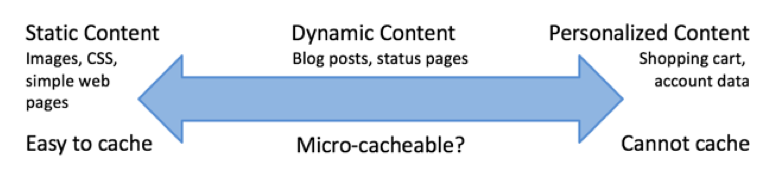
\includegraphics[width=5cm]{images/caching}
  \caption{HTMl Dokument einer React Seite}
\end{figure}

\subsection{Clientseitige Hydration}
\label{subsec:Clientseitige Hydration}

\begin{figure}[h]
  \centering
  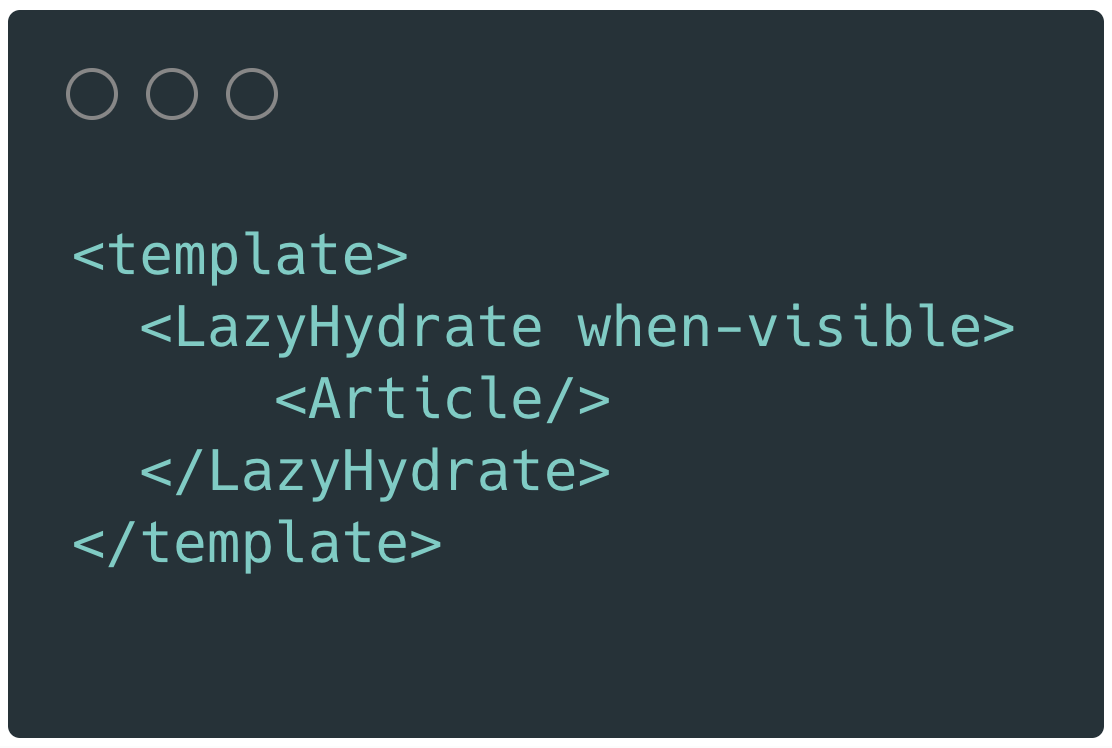
\includegraphics[width=5cm]{images/LazyHydration}
  \caption{HTMl Dokument einer React Seite}
\end{figure}

\subsection{Rendering Ablauf}
\label{subsec:Rendering Ablauf}

\begin{figure}[h]
  \centering
  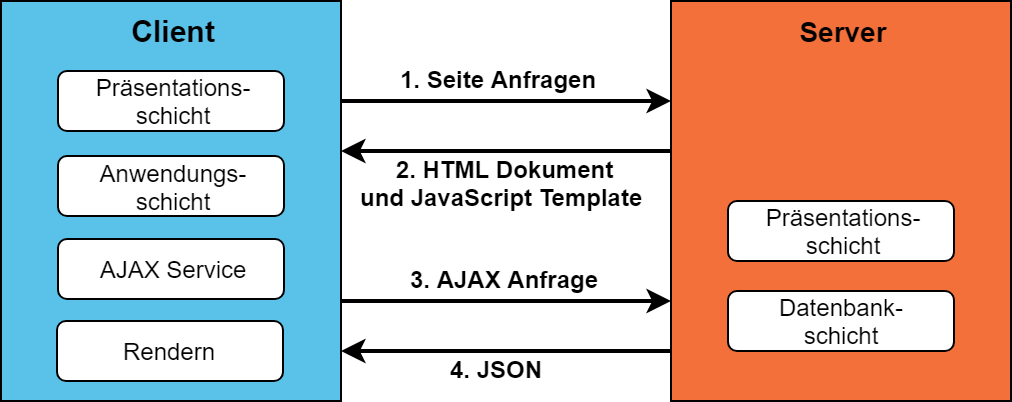
\includegraphics[width=12cm]{images/universal}
  \caption{HTMl Dokument einer React Seite}
\end{figure}

\newpage
\subsection{Vorteile}
\label{subsec:Vorteile}

\begin{figure}[h]
  \centering
  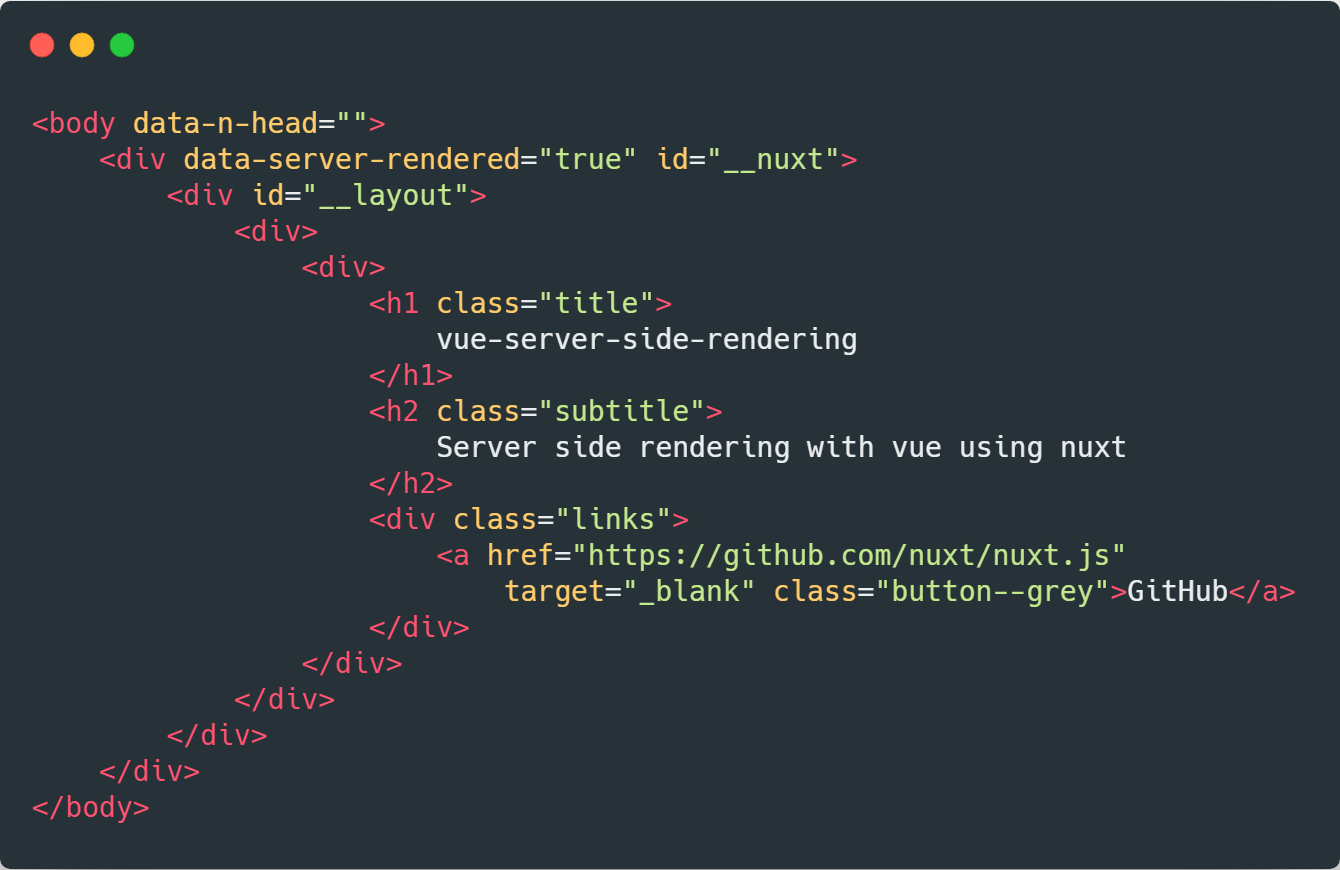
\includegraphics[width=9cm]{images/nuxt-body-first}
  \caption{HTMl Dokument einer React Seite}
\end{figure}

\subsection{Nachteile}
\label{subsec:Nachteile}

\subsection{Alternativen}
\label{subsec:Alternativen}

\begin{figure}[h]
  \centering
  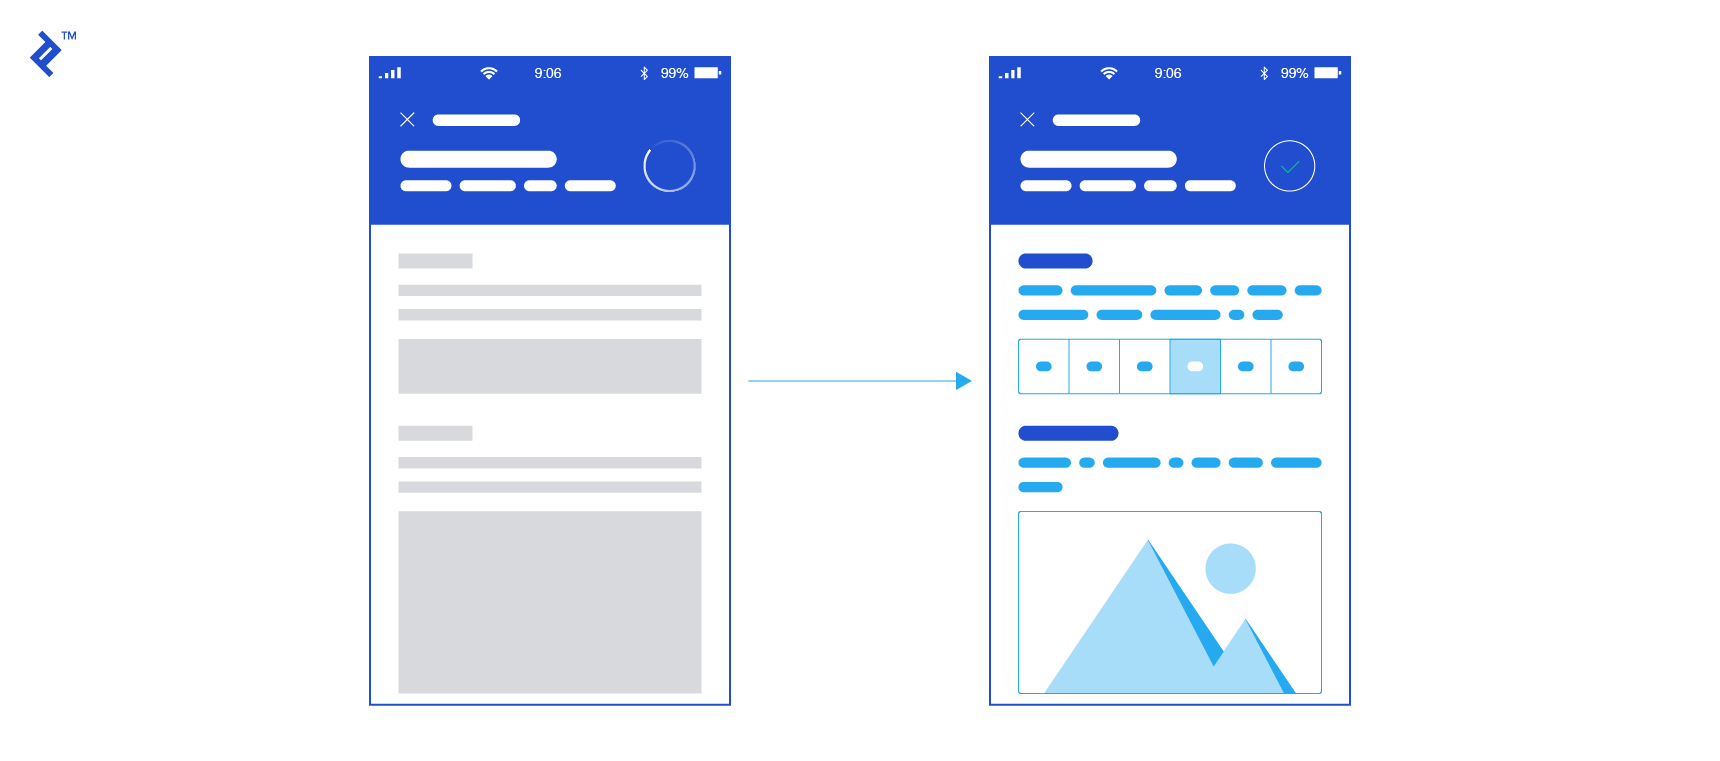
\includegraphics[width=9cm]{images/WebsiteSceleton}
  \caption{HTMl Dokument einer React Seite}
\end{figure}

\newpage
% -------------------------------------------------------------------------------------------------

\section{Frameworks}
\label{sec:Evaluation}

\subsection{React und Next.js}
\label{subsec:React und Next.js}

\begin{figure}
  \centering
  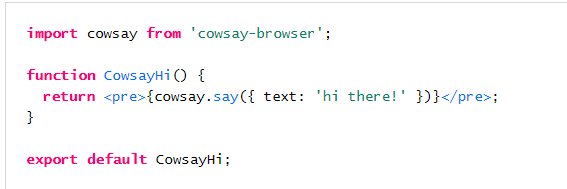
\includegraphics[width=10cm]{images/CodeSplitting}
  \caption{HTMl Dokument einer React Seite}
\end{figure}

\begin{figure}
  \centering
  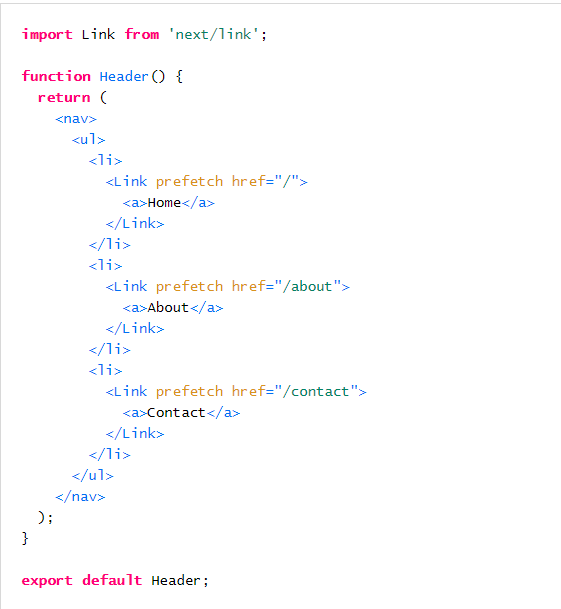
\includegraphics[width=7cm]{images/prefetchnext}
  \caption{HTMl Dokument einer React Seite}
\end{figure}


\subsection{Vue.js und Nuxt.js}
\label{subsec:Vue.js und Nuxt.js}

\subsection{Angular Universal}
\label{subsec:Angular Universal}

\newpage
% -------------------------------------------------------------------------------------------------

\section{Universal Rendering in der Praxis}
\label{sec:Universal Rendering in der Praxis}

\newpage
% -------------------------------------------------------------------------------------------------

\section{Fazit und Ausblick}
\label{sec:Fazit}

\begin{figure}
  \centering
  
\includegraphics[width=10cm]{images/HackerNews}
  \caption{HTMl Dokument einer React Seite}
\end{figure}

\begin{figure}
  \centering
  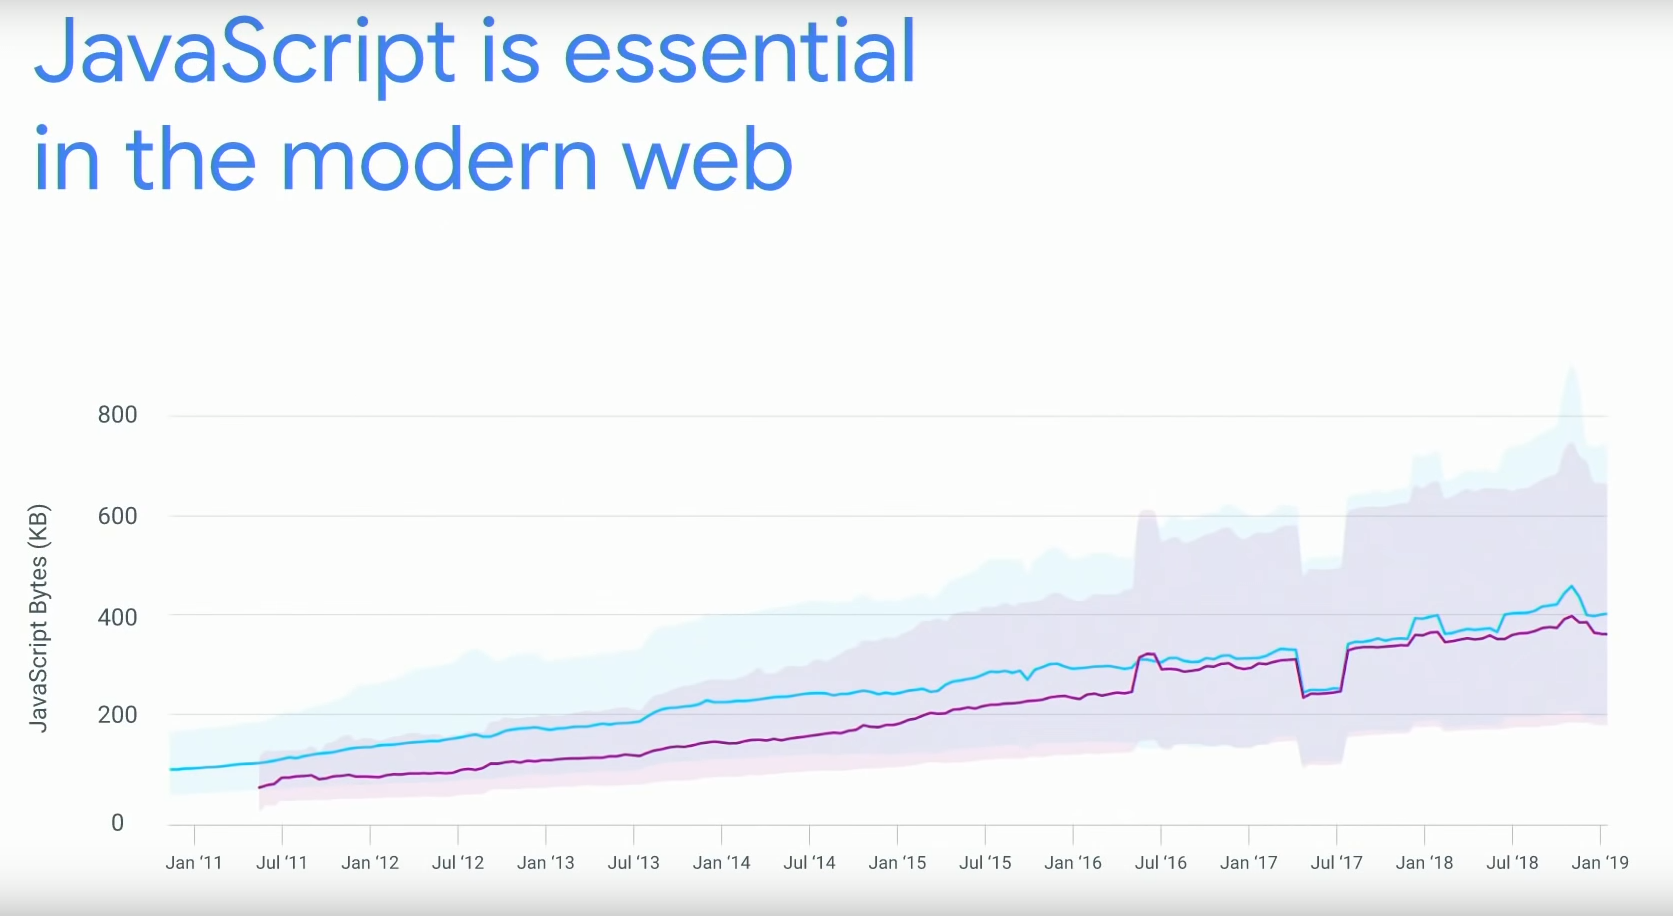
\includegraphics[width=10cm]{images/JavaScriptGoogleShips}
  \caption{HTMl Dokument einer React Seite}
\end{figure}




% -------------------------------------------------------------------------------------------------
\newpage
% Normaler LNCS Zitierstil
%\bibliographystyle{splncs}
\bibliographystyle{itmalpha}
% TODO: Ändern der folgenden Zeile, damit die .bib-Datei gefunden wird
\bibliography{literatur}

\end{document}
